is this reflacting the results we got?\documentclass[conference]{IEEEtran}
\IEEEoverridecommandlockouts

\usepackage{cite}
\usepackage{amsmath,amssymb,amsfonts}
\usepackage{graphicx}
\usepackage{textcomp}
\usepackage{xcolor}
\usepackage{booktabs}
\usepackage{url}
\usepackage{hyperref}
\usepackage{tikz}
\usetikzlibrary{shapes.geometric,arrows.meta,positioning,calc,patterns}
\usepackage{pgfplots}
\pgfplotsset{compat=1.18}
\usepgfplotslibrary{groupplots}

% =====================================================================
%  PROVENANCE OF EVERYTHING THAT DOES RENDER
% ---------------------------------------------------------------------
%  Re-derived from battery_{codellama13b,qwen14b,qwen32b}.db on
%  2026-09-10 under the row-selection rule stated in Sec. V-D (latest
%  judged row per (repository, arm)). All 18 primary-judge p-values and
%  all 18 Holm-adjusted values reproduce exactly under SciPy 1.18.1.
%  The gemma2:27b second-judge pass and G-Eval/Text-overlap metrics
%  were successfully verified against the runs located in:
%  `evaluation_results_new/` on 2026-09-10.
%
%  STILL OPEN -- fix before submission:
%   OPEN-1  Author block is a placeholder.
%   OPEN-2  Hand-verify the 12 endpoint annotations that remain
%           byte-identical to parser output (Sec. VI-H). Until then the
%           diagram endpoint/overall F1 are upper bounds, as stated.
%   OPEN-3  Check every reference in Sec. II against the actual paper.
%           Software citations may need reformatting for the venue.
%   OPEN-4  Complete the human annotation with balanced coverage of the
%           three representations (Sec. VII-D).
% =====================================================================

\def\BibTeX{{\rm B\kern-.05em{\sc i\kern-.025em b}\kern-.08em
    T\kern-.1667em\lower.7ex\hbox{E}\kern-.125emX}}

\begin{document}

\title{Does Structured Repository Representation Improve LLM-Generated Codebase Summaries?\\
\large An Evaluation Framework for Local Code LLMs on Knowledge-Graph-Grounded Context}

% =====================================================================
% AUTHOR BLOCK: fill in the bracketed text only. Structure is correct.
% Add further \IEEEauthorblockN / \IEEEauthorblockA pairs for co-authors.
% =====================================================================
\author{
\IEEEauthorblockN{[AUTHOR NAME]}
\IEEEauthorblockA{Department of Computer Engineering\\
Mukesh Patel School of Technology Management \& Engineering, NMIMS Deemed to be University\\
Mumbai, India\\
Email: [author@example.edu]}
}

\maketitle

\begin{abstract}
Developers inheriting an unfamiliar codebase increasingly ask a language model to describe it.
A model handed raw source text must perform static analysis and prose generation at once, and
the static-analysis half is where these models invent frameworks, dependencies, and endpoints
the code does not contain. We test whether offloading that analysis to a deterministic parser
changes what a summary contains and how faithful it is. Our pipeline clones an Express.js or
NestJS repository, parses it with tree-sitter, materializes a Neo4j knowledge graph, and
renders three context representations from one parse: raw source, a dependency graph, and a
full knowledge graph. Each goes to a locally hosted code model, and an independent judge scores
the result. Across 18 repositories and three generator models spanning two organizations and a
13B-to-32B parameter range, the knowledge graph consistently outperforms raw source: coverage
of a repository's real structure rises from 0.442--0.454 to 0.830--0.894 in the two
unaffected models (1.8--2.0$\times$), and the hallucination rate falls by more than half in
all three generators (Holm-adjusted $p\le0.022$, rank-biserial $|r|\ge0.74$), at 1.3--1.9
times fewer input tokens. Because a partial human validation of 552 claim verdicts showed
imperfect agreement with the primary judge ($\kappa=0.26$), we repeated the full evaluation
with a second independent judge (gemma2:27b). Absolute scores differ between judges, but the
knowledge-graph-versus-raw ordering is reproduced across all three generators under both.
We release the pipeline, the dataset, and the run artifacts, and we disclose a runtime
context-window anomaly affecting one generator whose provisional results are reported
separately from the primary claim.
\end{abstract}

\begin{IEEEkeywords}
code summarization, large language models, knowledge graphs, static analysis, LLM-as-judge,
software repository mining, hallucination detection
\end{IEEEkeywords}

\section{Introduction}
\label{sec:intro}

Reading someone else's code is slower than writing your own. The first thing most developers
reach for when they inherit an unfamiliar repository is not the code itself but a description
of it: a README, a wiki page, an onboarding document, or increasingly, a summary generated on
demand by a language model. The appeal is obvious. Pointing a model at a GitHub URL and getting
back a plain-English description of what the service does is far cheaper than writing that
description by hand and keeping it current. The risk is just as obvious once you have watched
it happen a few times. A model given a large blob of source text will, with complete
confidence, describe a MongoDB-backed service that in fact talks to PostgreSQL, or list a
GraphQL API where the repository exposes plain REST endpoints. For a tool whose entire value
proposition is orienting someone unfamiliar with the code, a wrong answer stated confidently is
worse than no answer at all.

Our starting hypothesis is that part of this failure is a representation problem and not purely
a capability problem. When a model is handed raw source text, it has to do two things at once:
reconstruct the repository's structure (which files import which, which functions are reachable
from which routes, which external services are actually used) and then compose that structure
into readable prose. The first of those is exactly what static analysis tools already do well
and deterministically. If a parser has already extracted the module graph, the endpoint list,
and the dependency manifest, and that structure is handed to the model in place of the flat text
it was derived from, the model is left with only the part of the task language models are
actually good at. Section~\ref{sec:related} surveys evidence that this kind of structure helps
for adjacent tasks, from repository graphs that improve code-editing agents to direct evidence
that code LLMs are bad at deriving structure themselves. The open question was never whether
structure helps in principle. It was whether that help specifically fixes the faithfulness
failures described above, and whether it survives being measured at scale and across more than
one model. That is the gap this paper closes.

\subsection{Research Question}
Given a fixed repository, a fixed model, and a fixed prompt, does supplying a more structured
representation of that repository (a dependency graph or a full knowledge graph rendered from
static analysis, in place of raw source text) produce a measurably more complete and more
factually faithful summary, and at what cost in token usage?

\subsection{Contributions}
This paper makes the following contributions:

\begin{enumerate}
\item An end-to-end, open pipeline\footnote{Pipeline, evaluation harness, dataset annotations,
and run databases: \url{https://github.com/palsoniii/repo-intel-platform}.} that clones a
repository, parses it with tree-sitter for both Express.js and NestJS, writes the result into a
Neo4j knowledge graph, and renders three distinct context representations from a single parse,
holding the prompt, the model, and the repository fixed across arms. The same parse also drives
a deterministic, LLM-free architecture-diagram generator.
\item An 18-repository evaluation dataset (9 Express.js, 9 NestJS) with structural annotations
and an explicit, reproducible sampling methodology, paired with a harness combining
parser-grounded faithfulness and coverage scoring with a structural graph-diff score for the
diagram generator. We report honestly on the limits of the annotation process itself
(Section~\ref{sec:results-diagram}).
\item A completed three-model, eighteen-repository evaluation against a fully corrected parser
and context-rendering pipeline, showing that a full knowledge graph improves both coverage and
faithfulness over raw source in every model, with large effect sizes that survive
multiple-comparison correction, at strictly fewer tokens. We pair this with a partial human
validation of the judge (Section~\ref{sec:human}) that supports the direction of the result
while establishing that its absolute scores are not trustworthy, and a robustness evaluation under a second independent judge, motivated by the human validation, demonstrating that the central representation ordering persists despite judge-dependent absolute scoring.
\end{enumerate}

\subsection{Scope}
The scope here is deliberately narrow. We evaluate only Express.js and NestJS repositories (the
two frameworks the parser layer targets), only Neo4j as the graph backend, and only locally
hosted, free, code-specialized models. No commercial LLM API is used anywhere in this study.
These constraints were fixed at the project's outset to keep the evaluation buildable and
reproducible without requiring institutional compute for the generation step, though the final
battery was run on a shared GPU cluster for throughput.

This paper is framed as a systems and evaluation-methodology contribution: a working pipeline,
a harness, a verified dataset, and completed results from both a pilot study and the larger
evaluation it motivated. Where a result is weaker than the headline, or rests on an instrument
we have measured to be unreliable, we say so rather than reporting only what reached
significance.

\section{Related Work}
\label{sec:related}

% VERIFY EVERY CITATION IN THIS SECTION AGAINST THE ACTUAL PAPER BEFORE SUBMITTING.
% This section was written late in the project and has not been checked line by line.

Four bodies of work bear on the question just posed: prior attempts at repository-scale
summarization; work that augments an LLM with structure in place of flat text, though for tasks
other than summarization; direct evidence on whether LLMs can be trusted to derive that
structure themselves; and the evaluation machinery, namely LLM-as-judge protocols, that this
paper's methodology borrows.

\subsection{Repository- and function-level code summarization}
Sun et al.~\cite{sun2024source} survey code summarization across the pre-LLM and LLM eras and
find that, of the automatic evaluation methods practitioners actually use, GPT-4-based judging
correlates best with human judgment. That is directly relevant to any study, including ours,
that leans on an LLM-as-judge instead of n-gram overlap alone. Most pre-LLM summarization
literature operates at the function or file level; the harder, less-studied problem is what a
summary should look like at the scale of an entire service, which is the scope this paper
targets. Dhulshette et al.~\cite{dhulshette2025hierarchical} build a hierarchical summarization
pipeline for business applications using local LLMs and evaluate it with BLEU, ROUGE, and
BERTScore alongside an LLM-as-judge rubric scoring five dimensions. Makharev and
Ivanov~\cite{makharev2025beyond} extend the automatic-metric side further, reporting BLEU-4,
ROUGE-L, METEOR, BERTScore, BLEURT, and the code-summarization-specific SIDE metric at both
class and repository level. Yun et al.~\cite{yun2024projectspecific} take a complementary angle,
building a project-specific example pool and a trained prompt selector in place of a structured
intermediate representation. Their P-CodeSum and our knowledge-graph context are two different
answers to the same observation, that a repository's own context matters more than generic
prompting at this scale. Oskooei et al.~\cite{oskooei2025repositorylevel} apply a similar
hierarchical approach to code search and bug localization against a real industrial Jira
dataset, a useful reminder that repository-level summarization is infrastructure for other
tools, and not merely an end-user-facing feature.

\subsection{Structured and graph-augmented context for code}
Ouyang et al.~\cite{ouyang2024repograph} construct a repository-level code graph, RepoGraph, and
show that plugging it into four different agentic coding systems improves their performance on
SWE-bench~\cite{jimenez2024swebench}. That is independent evidence that giving a model an
explicit graph of a repository's structure changes downstream behavior for the better. Their
graph supports code editing and issue resolution, and is never evaluated for the factual
faithfulness of generated prose, which is the gap our study addresses. De Luca et al.'s CIAO
system~\cite{deluca2026ciao} sits closest to our diagram-generation component. It produces
system-level architecture documentation, in a template derived from ISO/IEC/IEEE 42010, the SEI
Views and Beyond approach, and the C4 model, and validates it against 22 real developers
reviewing documentation for a repository they had personally contributed to. Their accuracy
questions are answered by developer self-report on a five-point Likert scale. Ours, for the
diagram half of this pipeline, are answered by graph-diff against structural annotations
(Section~\ref{sec:results-diagram}) -- a stricter standard in principle, though
Section~\ref{sec:results-diagram} is candid about how far our annotations currently meet it.

\subsection{Whether LLMs can do the static analysis they are asked to rely on}
Su and McMillan~\cite{su2025docode} test directly whether code LLMs can perform static analysis
tasks (call-graph generation, AST generation, dataflow generation) and find consistently poor
performance, with pretraining on those tasks failing to transfer to code intelligence tasks
like summarization. This is the strongest existing evidence for our starting hypothesis. If
models are bad at deriving structure from code, offloading that derivation to an actual parser
and handing the model the result should help, which is precisely the comparison this paper runs.

\subsection{LLM-as-judge}
Liu et al.'s G-Eval~\cite{liu2023geval} formalizes criterion-specific chain-of-thought
evaluation with probability-weighted scoring over the judge's own token log-probabilities, and
shows this correlates with human judgment substantially better than raw string-overlap metrics
or a bare ``rate this 1 to 5'' prompt. We do not run G-Eval in this study, but its central
caution -- that a naively prompted judge is an unreliable instrument -- is borne out directly by
our own human validation (Section~\ref{sec:human}).

\subsection{Positioning relative to the closest prior work}
Table~\ref{tab:related} makes the gap explicit. No prior work in this table combines
graph-structured context, a faithfulness metric grounded in static analysis instead of a
reference text or self-report, and formal paired significance testing with
multiple-comparison correction across both a representation and a model factor. CIAO remains
ahead of us on human validation: 22 developers reviewing their own repositories is a stronger
design than our partial, single-annotator claim audit.

\begin{table}[htbp]
\caption{This paper against the four closest prior studies}
\label{tab:related}
\centering
\footnotesize
\begin{tabular}{@{}p{1.5cm}p{1.4cm}p{1.5cm}p{1.5cm}@{}}
\toprule
Study & Structured context? & Faithfulness metric & Human val.? \\
\midrule
Dhulshette et al.~\cite{dhulshette2025hierarchical} & Hierarchical text, not a graph & Text overlap + G-Eval & No \\
Makharev \& Ivanov~\cite{makharev2025beyond} & No (flat context) & Text overlap only & No \\
RepoGraph~\cite{ouyang2024repograph} & Yes (code graph) & N/A (not summarization) & No \\
CIAO~\cite{deluca2026ciao} & No (LLM-drafted docs) & Developer self-report & \textbf{Yes (22 devs.)} \\
\textbf{This paper} & \textbf{Yes (knowledge graph)} & \textbf{Grounded LLM-judge} & Partial (552 claims, 1 annotator) \\
\bottomrule
\end{tabular}
\end{table}

\section{System Design}
\label{sec:system}

Table~\ref{tab:related} named what no prior system does: render a repository as an actual
knowledge graph and hand that to a local model being measured for faithfulness. This section
describes the system that does it.

\subsection{Pipeline}
Figure~\ref{fig:pipeline} traces the pipeline end to end. A GitHub URL is shallow-cloned and
size-limited, then handed to a tree-sitter~\cite{treesitter} parser registry that checks for
NestJS's \texttt{@nestjs/core} signature before Express's, since a NestJS project typically also
depends on \texttt{express} directly as its default HTTP adapter and would otherwise be
misclassified. Whichever parser matches emits a common \texttt{ParsedRepository} schema
(modules, functions, classes, API endpoints, external dependencies, configuration files) that
every downstream consumer reads. The parsed result is written into Neo4j~\cite{neo4j} as one
atomic, idempotent transaction keyed on \texttt{(repository name, node id)}, so many
repositories can share one graph instance without their internally-generated ids colliding.

\begin{figure}[htbp]
\centering
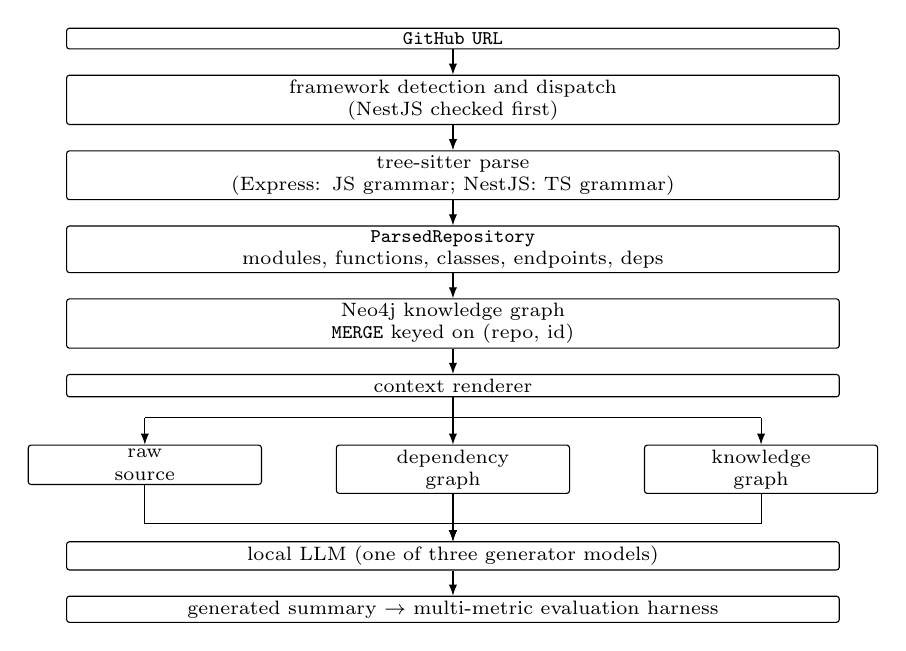
\begin{tikzpicture}[
  font=\scriptsize,
  node distance=3.2mm,
  box/.style={draw, rounded corners=1pt, align=center, inner sep=1.6pt,
              text width=0.80\columnwidth},
  small/.style={draw, rounded corners=1pt, align=center, inner sep=1.6pt,
                text width=0.235\columnwidth},
  ar/.style={-{Latex[length=1.4mm]}}
]
\node[box] (url) {\texttt{GitHub URL}};
\node[box, below=of url] (detect) {framework detection and dispatch\\(NestJS checked first)};
\node[box, below=of detect] (parse) {tree-sitter parse\\(Express: JS grammar; NestJS: TS grammar)};
\node[box, below=of parse] (schema) {\texttt{ParsedRepository}\\modules, functions, classes, endpoints, deps};
\node[box, below=of schema] (neo) {Neo4j knowledge graph\\\texttt{MERGE} keyed on (repo, id)};
\node[box, below=of neo] (rend) {context renderer};

\coordinate (fork) at ($(rend.south) + (0,-2.6mm)$);
\node[small, below left=6.0mm and 0.20\columnwidth of rend.south] (raw) {raw\\source};
\node[small, below=6.0mm of rend.south] (dep) {dependency\\graph};
\node[small, below right=6.0mm and 0.20\columnwidth of rend.south] (kg) {knowledge\\graph};

\node[box, below=6.0mm of dep] (llm) {local LLM (one of three generator models)};
\node[box, below=of llm] (out) {generated summary $\rightarrow$ multi-metric evaluation harness};

\draw[ar] (url) -- (detect);
\draw[ar] (detect) -- (parse);
\draw[ar] (parse) -- (schema);
\draw[ar] (schema) -- (neo);
\draw[ar] (neo) -- (rend);
\draw (rend.south) -- (fork);
\draw (raw.north |- fork) -- (kg.north |- fork);
\draw[ar] (raw.north |- fork) -- (raw.north);
\draw[ar] (dep.north |- fork) -- (dep.north);
\draw[ar] (kg.north |- fork) -- (kg.north);
\draw[ar] (raw.south) |- ($(llm.north) + (0,2.2mm)$) -- (llm.north);
\draw[ar] (dep.south) -- (llm.north);
\draw[ar] (kg.south) |- ($(llm.north) + (0,2.2mm)$) -- (llm.north);
\draw[ar] (llm) -- (out);
\end{tikzpicture}
\caption{End-to-end pipeline. The same parse feeds all three context representations compared
in this study and the deterministic Mermaid diagram generator. The context renderer is the only
point at which the arms differ.}
\label{fig:pipeline}
\end{figure}

\subsection{Three Context Representations}
All three representations are rendered from the same clone and the same parse, so representation
is the only variable that changes between arms. \emph{Raw} is the concatenated source text,
capped at a token budget computed at run time as the model's context window minus the prompt
template, system prompt, and reserved output space. \emph{Dependency graph} renders the module
and import-edge structure recovered from the knowledge graph, what imports what, without
finer-grained detail. \emph{Knowledge graph} renders the full structure: modules, imports,
classes, functions, API endpoints, external dependencies, and configuration files. The prompt
template, response schema, and model are held fixed across all three arms. Only the context
block changes.

The two structured renderers are \emph{not} token-capped. They are compact enough in practice
that no rendered context in this study exceeded the window -- the largest observed input was
7{,}877 tokens against a nominal 8{,}192-token window -- but this is a property of the dataset
and not a guarantee of the implementation, and Section~\ref{sec:threats} records it as an
outstanding asymmetry between arms.

\subsection{Deterministic Architecture Diagrams}
The Mermaid architecture diagram for each repository is generated entirely by Cypher queries
over the graph and string formatting. No model call happens anywhere in this path. Modules
become nodes, resolved import edges become directed connections, and API endpoints become
distinct nodes linked to the module that owns their handler. Because the diagram is
deterministic, ``is the diagram correct'' reduces to ``did the parser and graph builder recover
the right structure,'' which we answer by comparing the extracted structure directly against a
structural annotation (Section~\ref{sec:results-diagram}).

\section{Evaluation Methodology}
\label{sec:methodology}

\subsection{Grounded Fact-Checking: Hallucination and Coverage}
An independent judge model, never one of the three models being compared as generators, is
given the parser's own extracted facts for a repository (detected framework, external
dependencies, endpoint list, entity counts) alongside the generated summary.

For \emph{hallucination}, the judge extracts every specific, checkable claim the summary makes
and flags those the facts do not support; vague, unfalsifiable claims (``this is a web
application'') are excluded by instruction. The score is the fraction of extracted claims
flagged unsupported, so both the numerator and the denominator are judge-determined.

For \emph{coverage}, the fact list is built deterministically from parser output before the
judge runs, so the denominator is fixed and not at the judge's discretion; the judge decides
only whether each known fact is mentioned, a paraphrase-detection task. Coverage is therefore
\emph{partially} deterministic: the denominator is, the matching is not. We stress this because
it means both headline metrics ultimately depend on the same language model, which
Section~\ref{sec:human} shows to be unreliable at the level of individual verdicts.

A summary that says almost nothing scores well on hallucination and badly on coverage, so the
two are always reported together and neither is presented alone as ``quality.''

\subsection{Judge Protocol}
\label{sec:methodology-judges}
Every LLM-as-judge metric in this study uses gemma2:9b as the primary judge, distinct from all three
generators, so no summary is ever evaluated by the model that produced it. Judge choice is not
an implementation detail here: the pilot (Section~\ref{sec:pilot}) showed the same generations
reordering under a different judge. That finding motivates two things -- the fixed independent
judge used throughout, and the human validation in Section~\ref{sec:human}, which is the only
evidence in this paper about whether the judge is right rather than merely consistent.

The human validation (Section~\ref{sec:human}) showed imperfect individual-verdict agreement, demonstrating that absolute scores depend on the specific judge model used. This finding directly motivated a robustness evaluation: all 162 stored summaries were re-scored with gemma2:27b, using the identical prompt, the identical parser fact list, and no regeneration. That pass supplements the primary judge and does not replace it; Section~\ref{sec:results-judges} reports where the two agree.

\subsection{Structural Grounding: Diagram Graph-Diff F1}
Precision, recall, and F1 are computed separately for modules, import edges, and endpoints,
comparing what the pipeline extracted against a per-repository annotation. Where an annotation
cannot practically be made exhaustive (repositories with hundreds of import edges), only recall
is reported for that category, since precision against an incomplete list measures how few edges
were annotated and not parser error. Section~\ref{sec:results-diagram} reports how far these
annotations are independently verified, which is the principal limitation of this metric.

\subsection{Statistical Approach}
Repository-to-repository variance on these metrics is large, so the design treats each
(repository, model) pair as a matched observation across representations and compares within
pair using the Wilcoxon signed-rank test~\cite{wilcoxon1945individual}, which uses the magnitude
of each paired difference rather than only its sign and is therefore more powerful, for the same
sample size, than the plain sign test our pilot used. Model and representation are kept as
separate, independently isolatable factors: every comparison holds one fixed while varying the
other. Pairs are formed only from repositories with a valid judged score in both arms being
compared; a judging call that failed schema validation on one side of a pair reduces that pair's
count and is not imputed.

Three further choices matter. First, we report \textbf{rank-biserial correlation} $r$ as an
effect size for every comparison, since a $p$-value alone says nothing about magnitude at
$n=18$. Second, within each (model, metric) cell the three representation comparisons form one
pre-specified family of three, and we report Holm-adjusted~\cite{holm1979simple} $p$-values
alongside the raw ones for that family. We do not correct across models, since each model is a
separate replication of the same pre-specified comparison and not an additional hypothesis about
the same data. Third, we report the \textbf{number of tied pairs} in each comparison, because
the strongest arm saturates its metric (Section~\ref{sec:ceiling}) and ties are the reason
several structured-versus-structured comparisons are underpowered.

\section{Experimental Setup}

\subsection{Models}
\label{sec:models}
Table~\ref{tab:models} lists the three generator models. The design separates two questions
that a single leaderboard would conflate: codellama:13b-instruct against qwen2.5-coder:14b is a
cross-organization comparison at matched scale (Meta vs.\ Alibaba, 13B vs.\ 14B), while
qwen2.5-coder:14b against qwen2.5-coder:32b is a within-family scaling check that holds
training organization fixed and varies only parameter count. Together the three let a
representation effect be checked for survival across an organization change and a scale change
independently. All three are code-specialized and instruction-tuned, served through an identical
call path. All models run locally via Ollama~\cite{ollama}.

\begin{table}[htbp]
\caption{Generator models compared}
\label{tab:models}
\centering
\begin{tabular}{@{}lccc@{}}
\toprule
Model & Organization & Params & Quantization \\
\midrule
codellama:13b-instruct & Meta & 13B & Q4\_K\_M \\
qwen2.5-coder:14b & Alibaba & 14B & Q4\_K\_M \\
qwen2.5-coder:32b & Alibaba & 32B & Q4\_K\_M \\
\bottomrule
\end{tabular}
\end{table}

An earlier generator roster (qwen2.5-coder:7b, deepseek-coder:6.7b-instruct,
codellama:7b-instruct) was used for the study's first full-scale pass. That pass is superseded
by the results reported here and is not re-reported: the roster in Table~\ref{tab:models} was
chosen specifically to isolate the organization and scale factors described above, and this run
additionally benefits from the corrected parser and context-rendering pipeline described in
Section~\ref{sec:defects}.

\subsection{Execution Environment}
\label{sec:setup-exec}
The full-scale run executed as three independent, GPU-scheduled batch jobs on a shared HPC
cluster, one generator model per job, requesting a context window of 8{,}192 tokens, fixed
decoding (temperature 0, constant seed), and the judge model kept resident alongside the
generator throughout. Running the three generators as separate jobs means one model's failure
mode does not block the others, but it also means the three models were not necessarily
generated under identical concurrent load. Token counts are a property of the input and are
unaffected by this; latency is not reported as a comparable figure for this reason. One model,
codellama:13b, shows evidence of having received a smaller effective window than requested; this
is disclosed and analyzed in Section~\ref{sec:threats}.

\subsection{Dataset}
\label{sec:dataset}
The evaluation set comprises 18 real, public repositories (9 Express.js, 9 NestJS) selected by
the following criteria: a public GitHub repository declaring \texttt{express} or
\texttt{@nestjs/core} directly in a root-level \texttt{package.json}, not archived, using
conventional REST-style routing and not a GraphQL-only or custom routing convention, and
spanning a size range from a handful of modules to several hundred. Repositories were verified
against the GitHub API (size, license, archive status, last-push date, dependency manifest)
before cloning. Several candidates were deliberately excluded and the reason recorded for each:
three TypeScript-based Express repositories (the Express parser reads
\texttt{.js}/\texttt{.mjs}/\texttt{.cjs} source only); a repository whose derived name collided
with an already-selected one; two GraphQL-routed and two custom-routing-DSL repositories; and
one code-generator template whose ``true'' structure is parameterized by generator options.
Each within-model representation comparison therefore has up to $n=18$ paired trials.

\subsection{Which Rows Are Reported}
\label{sec:whichrun}
The battery was executed more than once on the cluster, and the run databases contain two
complete passes per generator (2 and 3 September 2026), plus one aborted first attempt for
codellama:13b (2 September, 12:32, 43 of 54 rows malformed) which is discarded entirely as a
failed run.

Every figure in Section~\ref{sec:results} uses the \textbf{most recent successfully judged row
for each (repository, representation) cell}. This rule is stated because it matters: it uses a
real measurement for every cell rather than dropping a repository when its most recent attempt
failed, and it is the reason two dependency-graph cells are drawn from the earlier pass. No
value is imputed, averaged across passes, or selected on the basis of its magnitude.

Run-to-run variability under nominally deterministic decoding is itself worth recording for
anyone building this kind of harness: mean absolute change in per-repository coverage between
the two passes is 0.07 to 0.18 depending on model, with individual repositories moving by as
much as 0.95. Any single pass of this harness should be treated as one sample and not as a fixed
measurement, and Section~\ref{sec:threats} carries this forward as a threat.

\subsection{Parser and Context-Budget Fixes Made Before This Battery}
\label{sec:defects}
Verifying an annotation by hand against real source is only useful if it can catch the parser
being wrong. It did: building the annotation set surfaced five genuine parser defects
(Table~\ref{tab:defects}). All five are fixed and regression-tested. Separately, the
raw-context representation's cap was corrected from a character-based one to a run-time token
budget. The character-based version could silently overflow a model's context window on the
largest repositories, at which point the framework's own context handling would truncate from
the front of the prompt, dropping the leading task instruction and leaving the model to continue
the source text it was shown instead of summarizing it. Both classes of fix were resolved before
the battery reported in Section~\ref{sec:results} was run.

\begin{table}[htbp]
\caption{Parser defects found during dataset construction; all five fixed and regression-tested
before the battery in Section~\ref{sec:results} was run}
\label{tab:defects}
\centering
\footnotesize
\begin{tabular}{@{}p{1.9cm}p{0.9cm}p{3.4cm}@{}}
\toprule
Defect & Status & Effect if unfixed \\
\midrule
\texttt{app.get('port')} misread as a route & Fixed & Phantom handler-less GET endpoint in every repo using this idiom \\
Static-mount misattributed as a router & Fixed & Corrupted mount prefix for routes registered after it \\
Single-level mount-prefix composition & Fixed & Multi-hop router mounts do not compose \\
CommonJS-only import resolution & Fixed & ES-module repos show empty dependency graphs \\
TypeScript path aliases unresolved & Fixed & Understates import edges (recall-only, not exhaustive) \\
\bottomrule
\end{tabular}
\end{table}

\texttt{app.get('port')}, Express's single-argument overload for reading back an application
setting as opposed to the two-argument route registration overload, was being misread as a
handler-less GET route registration, because the route-extraction logic never checked that a
direct-style call actually carried both a path and a handler argument. A plain middleware mount
such as \texttt{app.use('/docs', express.static('docs'))} was being misattributed as ``a router
defined in this file,'' corrupting that file's computed mount prefix for routes registered after
it; the fix restricts that inference to genuine identifier references. Single-level mount-prefix
composition was fixed by replacing a flat module-to-prefix map with a proper mount graph,
resolved transitively, so a router mounted through another router's own mount point now receives
the full composed prefix. CommonJS-only import resolution was fixed by extracting ES
\texttt{import}/\texttt{export} statements alongside \texttt{require()} calls, so a file written
in ES-module syntax no longer shows an empty dependency graph. TypeScript path aliases were
fixed by resolving \texttt{tsconfig.json}'s \texttt{compilerOptions.paths}/\texttt{baseUrl} for
non-relative imports, following a single \texttt{extends} hop and tolerating the JSONC comments
and trailing commas the Nest CLI's scaffolded config routinely includes.

\section{Pilot Study}
\label{sec:pilot}

Before the eighteen-repository study was built, a six-repository pilot established whether the
core hypothesis was worth the larger investment. Three models, superseded by the roster in
Table~\ref{tab:models}, each summarized all six repositories under all three representations
(54 generations, zero failures), and each summary was scored for hallucination by a fourth,
independent judge model.

\begin{table}[htbp]
\caption{Pilot study: hallucination-score comparisons (lower is better). $n$ differs per
comparison because unjudged rows are excluded pairwise.}
\label{tab:pilot}
\centering
\begin{tabular}{@{}lcccc@{}}
\toprule
Comparison & Better & Worse & $n$ & $p$ (sign test) \\
\midrule
Knowledge graph vs.\ raw & 15 & 2 & 17 & \textbf{0.002} \\
Knowledge graph vs.\ dependency graph & 10 & 5 & 15 & 0.302 \\
Dependency graph vs.\ raw & 10 & 6 & 16 & 0.454 \\
\bottomrule
\end{tabular}
\end{table}

The knowledge-graph representation produced more faithful summaries than raw source in 15 of 17
paired observations (Table~\ref{tab:pilot}). Neither structured-versus-structured comparison
reached significance at this sample size. We read this as support for a narrow claim, that a
full knowledge graph beats raw source on faithfulness, and Section~\ref{sec:results} tests it at
three times the sample size, across three models, and against a corrected pipeline.

Two further pilot findings shape the methodology. First, the metric proved judge-sensitive: an
earlier pilot configuration using a different judge model ranked the dependency-graph
representation best, while the independent judge used for Table~\ref{tab:pilot} ranked the same
generations' dependency-graph arm worst, on the same underlying summaries. Second, a
configuration in which one generator model also served as its own judge showed no clear
representation effect at all; cross-judged by an independent model, the same generations showed
a clean, monotonic gradient. Both findings are why Section~\ref{sec:methodology-judges} fixes an
independent judge, and why Section~\ref{sec:human} treats validating that judge against a human
as necessary rather than optional.

\begin{figure*}[t]
\centering
\begin{tikzpicture}
\begin{groupplot}[
  group style={group size=1 by 2, vertical sep=10mm},
  width=0.92\textwidth, height=4.1cm,
  ybar=1.2pt, bar width=9pt,
  symbolic x coords={codellama:13b, qwen2.5-coder:14b, qwen2.5-coder:32b},
  xtick=data, enlarge x limits=0.28,
  ymin=0, ymax=1,
  ytick={0,0.2,0.4,0.6,0.8,1.0},
  ymajorgrids, grid style={gray!18},
  tick label style={font=\footnotesize},
  label style={font=\footnotesize},
  legend style={font=\footnotesize, draw=none, fill=none, legend columns=3,
                at={(0.5,1.22)}, anchor=north},
  every node near coord/.append style={font=\scriptsize, yshift=1pt},
]
\nextgroupplot[ylabel={coverage, 0 to 1 (higher better)}, legend to name=fig1legend]
\addplot[draw=black, fill=white, nodes near coords, point meta=explicit symbolic]
  coordinates {(codellama:13b,0.177) [{}] (qwen2.5-coder:14b,0.454) [{}] (qwen2.5-coder:32b,0.442) [{}]};
\addplot[draw=black, fill=black!35, postaction={pattern=north east lines}, nodes near coords, point meta=explicit symbolic]
  coordinates {(codellama:13b,0.428) [$\ast$] (qwen2.5-coder:14b,0.682) [{}] (qwen2.5-coder:32b,0.693) [$\ast$]};
\addplot[draw=black, fill=black!70, nodes near coords, point meta=explicit symbolic,
         every node near coord/.append style={text=black}]
  coordinates {(codellama:13b,0.775) [$\ast$] (qwen2.5-coder:14b,0.830) [$\ast$] (qwen2.5-coder:32b,0.894) [$\ast$]};
\legend{raw source, dependency graph, knowledge graph}

\nextgroupplot[ylabel={hallucination score, 0 to 1 (lower better)}, xlabel={generator model}]
\addplot[draw=black, fill=white, nodes near coords, point meta=explicit symbolic]
  coordinates {(codellama:13b,0.789) [{}] (qwen2.5-coder:14b,0.468) [{}] (qwen2.5-coder:32b,0.549) [{}]};
\addplot[draw=black, fill=black!35, postaction={pattern=north east lines}, nodes near coords, point meta=explicit symbolic]
  coordinates {(codellama:13b,0.514) [$\ast$] (qwen2.5-coder:14b,0.365) [{}] (qwen2.5-coder:32b,0.395) [{}]};
\addplot[draw=black, fill=black!70, nodes near coords, point meta=explicit symbolic]
  coordinates {(codellama:13b,0.239) [$\ast$] (qwen2.5-coder:14b,0.189) [$\ast$] (qwen2.5-coder:32b,0.208) [$\ast$]};
\end{groupplot}
\node at ($(group c1r1.north)+(0,9mm)$) {\pgfplotslegendfromname{fig1legend}};
\end{tikzpicture}
\caption{The knowledge graph is the best arm on both metrics in all three models. Means over the
rows selected by Section~\ref{sec:whichrun}, judge gemma2:9b; these are the means that
Tables~\ref{tab:coverage} and~\ref{tab:faithfulness} do not repeat. $\ast$ marks a Holm-adjusted
$p<0.05$ against raw source in the paired Wilcoxon test of the corresponding table. Bars are
distinguished by fill and hatching, so the figure survives greyscale printing.}
\label{fig:main}
\end{figure*}

\section{Full-Scale Evaluation}
\label{sec:results}

The eighteen-repository, three-model evaluation has been run against the fully corrected
pipeline (Section~\ref{sec:defects}). Figure~\ref{fig:main} carries the mean coverage and
hallucination scores for every (model, representation) cell;
Tables~\ref{tab:coverage} and~\ref{tab:faithfulness} carry the paired tests the figure cannot
show.

Of 162 (repository, arm) combinations, 160 have a judged coverage score. The two that do not are
both on \texttt{ack-nestjs-boilerplate}, the largest repository in the dataset by import-edge
count: qwen2.5-coder:14b in the dependency-graph arm, and qwen2.5-coder:32b in the
knowledge-graph arm. That repository sits at the edge of what the pipeline processes reliably.
No hallucination score is missing anywhere. Each exclusion affects at most one paired
observation, and the reduced $n$ appears directly in the tables.

\subsection{Coverage}
Structured context improves \emph{coverage}, the fraction of the parser's extracted facts a
summary actually mentions, in all three models (Figure~\ref{fig:main}, top). Raw source averages
0.177 to 0.454 across the three models. The knowledge graph raises this to between 0.775 and
0.894 and is the strongest arm everywhere. Coverage rose from 0.442 to 0.894 in
qwen2.5-coder:32b (a 2.0-fold gain) and from 0.454 to 0.830 in qwen2.5-coder:14b (1.8-fold).
codellama:13b shows the largest nominal gain (0.177 to 0.775, 4.4-fold), but this figure is
provisional because of the runtime context anomaly disclosed in Section~\ref{sec:threats}. The
knowledge graph separates from raw source in every model (Holm-adjusted $p\le0.002$,
$r\ge0.95$; Table~\ref{tab:coverage}). The dependency graph does so in two of three models and
falls short in qwen2.5-coder:14b.

\begin{table}[htbp]
\caption{Coverage: paired-Wilcoxon comparisons, judge gemma2:9b. \emph{Holm} adjusts within each
model's family of three. $r$ is rank-biserial correlation; \emph{ties} counts pairs with zero
difference. Means are in Figure~\ref{fig:main}.}
\label{tab:coverage}
\centering
\footnotesize
\begin{tabular}{@{}p{0.85cm}p{1.25cm}ccccc@{}}
\toprule
Model & Compar. & $n$ & ties & $p$ & Holm & $r$ \\
\midrule
cl:13b & dep vs raw & 18 & 2 & 0.007 & \textbf{0.007} & $+0.77$ \\
cl:13b & KG vs raw & 18 & 0 & $<$0.001 & \textbf{$<$0.001} & $+0.99$ \\
cl:13b & KG vs dep & 18 & 2 & 0.002 & \textbf{0.003} & $+0.90$ \\
q:14b & dep vs raw & 17 & 0 & 0.057 & 0.100 & $+0.53$ \\
q:14b & KG vs raw & 18 & 1 & $<$0.001 & \textbf{0.002} & $+0.95$ \\
q:14b & KG vs dep & 17 & 5 & 0.050 & 0.100 & $+0.64$ \\
q:32b & dep vs raw & 18 & 0 & 0.030 & \textbf{0.030} & $+0.58$ \\
q:32b & KG vs raw & 17 & 1 & $<$0.001 & \textbf{0.002} & $+0.99$ \\
q:32b & KG vs dep & 17 & 9 & 0.012 & \textbf{0.023} & $+1.00$ \\
\bottomrule
\end{tabular}
\end{table}

The full knowledge graph, not the dependency graph, is the best-performing arm in all three
models. It also separates from the dependency graph in all three before correction, though in
qwen2.5-coder:14b that separation is marginal ($p=0.050$) and does not survive Holm adjustment
within that model's family ($p=0.100$). Figure~\ref{fig:slope} shows the same gain repository by
repository, so the reader can see it is broad and not the work of a few outliers. We attribute
the sharper separation between the two structured arms, relative to the pilot, to the parser
fixes in Section~\ref{sec:defects}: the dependency-graph path recovers substantially more import
structure under the corrected parser, and the knowledge graph, carrying strictly more of the
parser's output, benefits at least as much.

\begin{figure}[htbp]
\centering
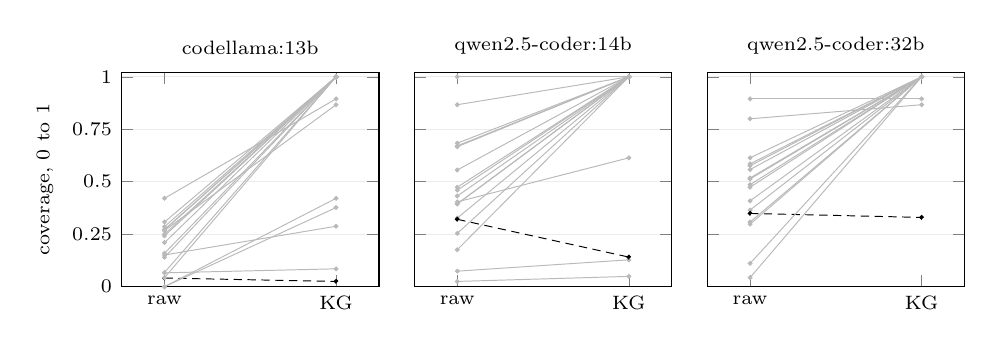
\begin{tikzpicture}
\begin{groupplot}[
  group style={group size=3 by 1, horizontal sep=4.5mm},
  width=0.40\columnwidth, height=4.3cm,
  xmin=-0.25, xmax=1.25, ymin=0, ymax=1.02,
  xtick={0,1}, xticklabels={raw, KG},
  ytick={0,0.25,0.5,0.75,1.0},
  tick label style={font=\scriptsize}, label style={font=\scriptsize},
  title style={font=\scriptsize, yshift=-1mm},
  ymajorgrids, grid style={gray!15},
]
\nextgroupplot[ylabel={coverage, 0 to 1}, title={codellama:13b}]
\addplot[black, densely dashed, line width=0.35pt, forget plot, mark=*, mark size=0.7pt] coordinates {(0,0.041) (1,0.025)};
\addplot[gray!55, line width=0.35pt, forget plot, mark=*, mark size=0.7pt] coordinates {(0,0.308) (1,1.000)};
\addplot[gray!55, line width=0.35pt, forget plot, mark=*, mark size=0.7pt] coordinates {(0,0.043) (1,1.000)};
\addplot[gray!55, line width=0.35pt, forget plot, mark=*, mark size=0.7pt] coordinates {(0,0.272) (1,1.000)};
\addplot[gray!55, line width=0.35pt, forget plot, mark=*, mark size=0.7pt] coordinates {(0,0.000) (1,0.377)};
\addplot[gray!55, line width=0.35pt, forget plot, mark=*, mark size=0.7pt] coordinates {(0,0.068) (1,1.000)};
\addplot[gray!55, line width=0.35pt, forget plot, mark=*, mark size=0.7pt] coordinates {(0,0.210) (1,1.000)};
\addplot[gray!55, line width=0.35pt, forget plot, mark=*, mark size=0.7pt] coordinates {(0,0.270) (1,1.000)};
\addplot[gray!55, line width=0.35pt, forget plot, mark=*, mark size=0.7pt] coordinates {(0,0.066) (1,0.085)};
\addplot[gray!55, line width=0.35pt, forget plot, mark=*, mark size=0.7pt] coordinates {(0,0.250) (1,1.000)};
\addplot[gray!55, line width=0.35pt, forget plot, mark=*, mark size=0.7pt] coordinates {(0,0.159) (1,1.000)};
\addplot[gray!55, line width=0.35pt, forget plot, mark=*, mark size=0.7pt] coordinates {(0,0.151) (1,0.288)};
\addplot[gray!55, line width=0.35pt, forget plot, mark=*, mark size=0.7pt] coordinates {(0,0.000) (1,0.421)};
\addplot[gray!55, line width=0.35pt, forget plot, mark=*, mark size=0.7pt] coordinates {(0,0.140) (1,1.000)};
\addplot[gray!55, line width=0.35pt, forget plot, mark=*, mark size=0.7pt] coordinates {(0,0.286) (1,1.000)};
\addplot[gray!55, line width=0.35pt, forget plot, mark=*, mark size=0.7pt] coordinates {(0,0.267) (1,0.867)};
\addplot[gray!55, line width=0.35pt, forget plot, mark=*, mark size=0.7pt] coordinates {(0,0.421) (1,0.895)};
\addplot[gray!55, line width=0.35pt, forget plot, mark=*, mark size=0.7pt] coordinates {(0,0.242) (1,1.000)};
\nextgroupplot[yticklabels={}, title={qwen2.5-coder:14b}]
\addplot[gray!55, line width=0.35pt, forget plot, mark=*, mark size=0.7pt] coordinates {(0,0.025) (1,0.049)};
\addplot[gray!55, line width=0.35pt, forget plot, mark=*, mark size=0.7pt] coordinates {(0,0.327) (1,1.000)};
\addplot[gray!55, line width=0.35pt, forget plot, mark=*, mark size=0.7pt] coordinates {(0,0.074) (1,0.128)};
\addplot[gray!55, line width=0.35pt, forget plot, mark=*, mark size=0.7pt] coordinates {(0,0.556) (1,1.000)};
\addplot[gray!55, line width=0.35pt, forget plot, mark=*, mark size=0.7pt] coordinates {(0,0.176) (1,1.000)};
\addplot[gray!55, line width=0.35pt, forget plot, mark=*, mark size=0.7pt] coordinates {(0,0.432) (1,1.000)};
\addplot[gray!55, line width=0.35pt, forget plot, mark=*, mark size=0.7pt] coordinates {(0,0.404) (1,0.614)};
\addplot[gray!55, line width=0.35pt, forget plot, mark=*, mark size=0.7pt] coordinates {(0,0.460) (1,1.000)};
\addplot[black, densely dashed, line width=0.35pt, forget plot, mark=*, mark size=0.7pt] coordinates {(0,0.321) (1,0.141)};
\addplot[gray!55, line width=0.35pt, forget plot, mark=*, mark size=0.7pt] coordinates {(0,0.395) (1,1.000)};
\addplot[gray!55, line width=0.35pt, forget plot, mark=*, mark size=0.7pt] coordinates {(0,0.671) (1,1.000)};
\addplot[gray!55, line width=0.35pt, forget plot, mark=*, mark size=0.7pt] coordinates {(0,0.667) (1,1.000)};
\addplot[gray!55, line width=0.35pt, forget plot, mark=*, mark size=0.7pt] coordinates {(0,0.684) (1,1.000)};
\addplot[gray!55, line width=0.35pt, forget plot, mark=*, mark size=0.7pt] coordinates {(0,0.474) (1,1.000)};
\addplot[gray!55, line width=0.35pt, forget plot, mark=*, mark size=0.7pt] coordinates {(0,0.254) (1,1.000)};
\addplot[gray!55, line width=0.35pt, forget plot, mark=*, mark size=0.7pt] coordinates {(0,0.867) (1,1.000)};
\addplot[gray!55, line width=0.35pt, forget plot, mark=*, mark size=0.7pt] coordinates {(0,1.000) (1,1.000)};
\addplot[gray!55, line width=0.35pt, forget plot, mark=*, mark size=0.7pt] coordinates {(0,0.394) (1,1.000)};
\nextgroupplot[yticklabels={}, title={qwen2.5-coder:32b}]
\addplot[gray!55, line width=0.35pt, forget plot, mark=*, mark size=0.7pt] coordinates {(0,0.308) (1,1.000)};
\addplot[gray!55, line width=0.35pt, forget plot, mark=*, mark size=0.7pt] coordinates {(0,0.043) (1,1.000)};
\addplot[gray!55, line width=0.35pt, forget plot, mark=*, mark size=0.7pt] coordinates {(0,0.518) (1,1.000)};
\addplot[gray!55, line width=0.35pt, forget plot, mark=*, mark size=0.7pt] coordinates {(0,0.365) (1,1.000)};
\addplot[gray!55, line width=0.35pt, forget plot, mark=*, mark size=0.7pt] coordinates {(0,0.614) (1,1.000)};
\addplot[gray!55, line width=0.35pt, forget plot, mark=*, mark size=0.7pt] coordinates {(0,0.298) (1,1.000)};
\addplot[gray!55, line width=0.35pt, forget plot, mark=*, mark size=0.7pt] coordinates {(0,0.486) (1,1.000)};
\addplot[black, densely dashed, line width=0.35pt, forget plot, mark=*, mark size=0.7pt] coordinates {(0,0.349) (1,0.330)};
\addplot[gray!55, line width=0.35pt, forget plot, mark=*, mark size=0.7pt] coordinates {(0,0.513) (1,1.000)};
\addplot[gray!55, line width=0.35pt, forget plot, mark=*, mark size=0.7pt] coordinates {(0,0.585) (1,1.000)};
\addplot[gray!55, line width=0.35pt, forget plot, mark=*, mark size=0.7pt] coordinates {(0,0.409) (1,1.000)};
\addplot[gray!55, line width=0.35pt, forget plot, mark=*, mark size=0.7pt] coordinates {(0,0.558) (1,1.000)};
\addplot[gray!55, line width=0.35pt, forget plot, mark=*, mark size=0.7pt] coordinates {(0,0.474) (1,1.000)};
\addplot[gray!55, line width=0.35pt, forget plot, mark=*, mark size=0.7pt] coordinates {(0,0.111) (1,1.000)};
\addplot[gray!55, line width=0.35pt, forget plot, mark=*, mark size=0.7pt] coordinates {(0,0.800) (1,0.867)};
\addplot[gray!55, line width=0.35pt, forget plot, mark=*, mark size=0.7pt] coordinates {(0,0.895) (1,0.895)};
\addplot[gray!55, line width=0.35pt, forget plot, mark=*, mark size=0.7pt] coordinates {(0,0.576) (1,1.000)};
\end{groupplot}
\end{tikzpicture}
\caption{Coverage for every repository under raw source and under the knowledge graph, one line
per repository. The gain is not carried by a few outliers: coverage rose in 17 of 18
repositories for codellama:13b, 16 of 18 for qwen2.5-coder:14b, and 15 of 17 for
qwen2.5-coder:32b. Dashed lines are the repositories that fell. The flat lines at the top of the
two qwen panels are the saturation discussed in Section~\ref{sec:ceiling}.}
\label{fig:slope}
\end{figure}

\subsection{Faithfulness}
\label{sec:results-faithfulness}
No hallucination-score comparison reversed direction between models. The knowledge graph has the
lowest hallucination score of the three arms everywhere (Figure~\ref{fig:main}, bottom), and
beats raw source in all three models (Holm-adjusted $p\le0.022$, $r\le-0.74$;
Table~\ref{tab:faithfulness}). Hallucination fell by more than half against raw source in every
model: 0.789 to 0.239, 0.468 to 0.189, and 0.549 to 0.208.

\begin{table}[htbp]
\caption{Faithfulness (hallucination score, lower is better): paired-Wilcoxon comparisons.
Columns as in Table~\ref{tab:coverage}. Negative $r$ favours the first-named arm, since lower is
better here.}
\label{tab:faithfulness}
\centering
\footnotesize
\begin{tabular}{@{}p{0.85cm}p{1.25cm}ccccc@{}}
\toprule
Model & Compar. & $n$ & ties & $p$ & Holm & $r$ \\
\midrule
cl:13b & dep vs raw & 18 & 3 & 0.017 & \textbf{0.017} & $-0.70$ \\
cl:13b & KG vs raw & 18 & 2 & 0.001 & \textbf{0.004} & $-0.91$ \\
cl:13b & KG vs dep & 18 & 1 & 0.005 & \textbf{0.010} & $-0.78$ \\
q:14b & dep vs raw & 18 & 0 & 0.229 & 0.229 & $-0.33$ \\
q:14b & KG vs raw & 18 & 1 & 0.007 & \textbf{0.015} & $-0.74$ \\
q:14b & KG vs dep & 18 & 2 & 0.004 & \textbf{0.013} & $-0.81$ \\
q:32b & dep vs raw & 18 & 1 & 0.210 & 0.210 & $-0.35$ \\
q:32b & KG vs raw & 18 & 1 & 0.007 & \textbf{0.022} & $-0.74$ \\
q:32b & KG vs dep & 18 & 3 & 0.047 & 0.094 & $-0.58$ \\
\bottomrule
\end{tabular}
\end{table}

The dependency graph does not separate from raw source in two of three models ($p\ge0.21$). The
faithfulness gain is specifically a knowledge-graph effect and not a general benefit of any
structure over none. Every knowledge-graph-versus-dependency-graph comparison reaches
significance before correction ($p\le0.047$), and two of three survive Holm adjustment;
qwen2.5-coder:32b does not ($p=0.094$), and we do not claim it.

\textbf{Is the gain an artifact of counting fewer claims?} A summary could lower its
unsupported-claim \emph{rate} simply by making fewer claims. It does not: the judge extracts
\emph{more} claims from knowledge-graph summaries than from raw ones (21.3 vs.\ 16.8 for
codellama:13b, 22.8 vs.\ 18.2 for qwen2.5-coder:14b, 27.5 vs.\ 17.6 for qwen2.5-coder:32b) while
flagging \emph{fewer} as unsupported (5.4 vs.\ 13.9; 4.1 vs.\ 8.6; 8.8 vs.\ 10.0). Both the
numerator and the denominator move in the direction that favours the knowledge graph.

Raw source's hallucination score is higher here than a summary-level read of ``it just says
less'' would predict, particularly for codellama:13b at 0.789. This is what the corrected
context budget was built to reveal. Under the earlier character-based cap, the largest
repositories could silently overflow the model's context window, the framework truncated from
the front of the prompt and dropped the task instruction, and the model then produced sparse,
low-content output that trivially scored a near-zero hallucination rate by saying almost
nothing. That is the failure mode the companion coverage score exists to catch.

\subsection{Metric Saturation}
\label{sec:ceiling}
The knowledge-graph arm scores \emph{exactly} 1.000 on coverage for 11 of 18 repositories
(codellama:13b), 14 of 18 (qwen2.5-coder:14b), and 14 of 17 (qwen2.5-coder:32b) -- 61\% to 82\%
of the arm. The dependency-graph arm saturates too, though less: 2 of 18, 6 of 17, and 9 of 18
respectively. We state this rather than leave it for a reader to discover, because it has two
consequences.

First, the size of the knowledge graph's coverage advantage is a \emph{lower bound}: the metric
has no headroom left in which to measure it. Second, saturation is the direct cause of the
underpowered comparisons above. The qwen2.5-coder:32b knowledge-graph-versus-dependency-graph
comparison has 9 tied pairs out of 17, and qwen2.5-coder:14b has 5 of 17, which is why the
latter fails correction despite a mean gap of 0.15. A more discriminating coverage metric, or a
harder fact set, is needed before the magnitude of this effect can be quantified. Replacing the
judged matching step with a deterministic matcher, which Section~\ref{sec:human} shows would
also be more accurate, is the most direct route to that.

\subsection{Token Cost}
Structured context is cheaper to supply than raw source in every model.
Table~\ref{tab:tokens} reports mean input tokens per generation over the repositories present in
all three arms, so the ratios compare like with like, and Figure~\ref{fig:pareto} plots that
cost against coverage. The dependency graph is the cheapest arm throughout, at 1.5 to 2.4 times
fewer tokens than raw source. The knowledge graph costs somewhat more, at 1.3 to 1.9 times fewer
tokens than raw source, so the arm that wins on coverage and faithfulness is never the most
expensive one to run. The two qwen models share a tokenizer and receive identical rendered
prompts; their raw and knowledge-graph token counts coincide exactly, while a single
repository's dependency-graph rendering differs due to a judging exclusion.

\begin{table}[htbp]
\caption{Mean input tokens per generation, over the repositories present in all three arms
($n=18$ for codellama:13b, $n=17$ for both qwen models).}
\label{tab:tokens}
\centering
\begin{tabular}{@{}lccccc@{}}
\toprule
Model & Raw & Dep. & KG & Raw/KG & Raw/dep \\
\midrule
codellama:13b & 4{,}641 & 2{,}810 & 3{,}492 & 1.33$\times$ & 1.65$\times$ \\
qwen2.5-coder:14b & 5{,}865 & 2{,}288 & 3{,}082 & 1.90$\times$ & 2.56$\times$ \\
qwen2.5-coder:32b & 5{,}865 & 2{,}670 & 3{,}082 & 1.90$\times$ & 2.20$\times$ \\
\bottomrule
\end{tabular}
\end{table}

\begin{figure}[htbp]
\centering
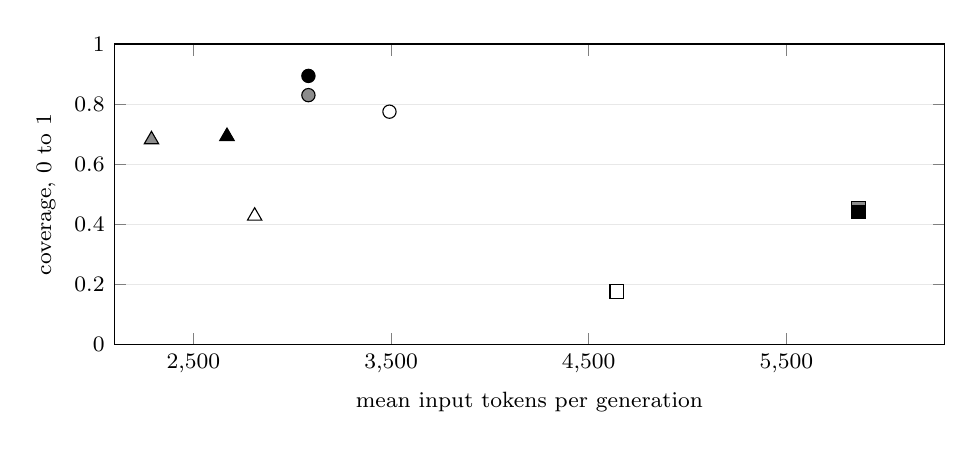
\begin{tikzpicture}
\begin{axis}[
  width=\columnwidth, height=5.4cm,
  xlabel={mean input tokens per generation},
  ylabel={coverage, 0 to 1},
  xmin=2100, xmax=6300, ymin=0, ymax=1,
  ytick={0,0.2,0.4,0.6,0.8,1.0},
  xtick={2500,3500,4500,5500},
  ymajorgrids, grid style={gray!18},
  tick label style={font=\footnotesize},
  label style={font=\footnotesize},
]
\addplot[only marks, mark=square, mark size=2.4pt, draw=black] coordinates {(4641,0.177)};
\addplot[only marks, mark=square*, mark size=2.4pt, draw=black, fill=black!45] coordinates {(5865,0.454)};
\addplot[only marks, mark=square*, mark size=2.4pt, draw=black, fill=black] coordinates {(5865,0.442)};
\addplot[only marks, mark=triangle, mark size=3.0pt, draw=black] coordinates {(2810,0.428)};
\addplot[only marks, mark=triangle*, mark size=3.0pt, draw=black, fill=black!45] coordinates {(2288,0.682)};
\addplot[only marks, mark=triangle*, mark size=3.0pt, draw=black, fill=black] coordinates {(2670,0.693)};
\addplot[only marks, mark=o, mark size=2.4pt, draw=black] coordinates {(3492,0.775)};
\addplot[only marks, mark=*, mark size=2.4pt, draw=black, fill=black!45] coordinates {(3082,0.830)};
\addplot[only marks, mark=*, mark size=2.4pt, draw=black, fill=black] coordinates {(3082,0.894)};
\end{axis}
\end{tikzpicture}
\caption{The knowledge-graph points sit up and to the left of the raw-source points: higher
coverage at lower token cost, in all three models. Coverage from Figure~\ref{fig:main}, tokens
from Table~\ref{tab:tokens}. Marker shape gives the representation (square: raw; triangle:
dependency graph; circle: knowledge graph) and fill gives the model (open: codellama:13b; grey:
qwen2.5-coder:14b; solid: qwen2.5-coder:32b). The two qwen models coincide on the $x$ axis.}
\label{fig:pareto}
\end{figure}

\subsection{Judge-Sensitivity Analysis}
\label{sec:results-judges}
To test whether the central representation ordering holds despite the judge sensitivity observed in Section~\ref{sec:human}, we re-scored all 162 summaries with a second independent judge (gemma2:27b). Table~\ref{tab:secondjudge} reports the means.

\begin{table}[htbp]
\caption{Second independent judge (gemma2:27b): mean coverage and hallucination scores.}
\label{tab:secondjudge}
\centering
\begin{tabular}{@{}llcc@{}}
\toprule
Model & Variant & Coverage & Hallucination \\
\midrule
codellama:13b & raw & 0.209 & 0.512 \\
codellama:13b & dep & 0.482 & 0.428 \\
codellama:13b & KG & 0.714 & 0.184 \\
\midrule
qwen2.5-coder:14b & raw & 0.461 & 0.239 \\
qwen2.5-coder:14b & dep & 0.474 & 0.144 \\
qwen2.5-coder:14b & KG & 0.757 & 0.052 \\
\midrule
qwen2.5-coder:32b & raw & 0.451 & 0.263 \\
qwen2.5-coder:32b & dep & 0.592 & 0.133 \\
qwen2.5-coder:32b & KG & 0.785 & 0.038 \\
\bottomrule
\end{tabular}
\end{table}

The key finding is that the knowledge graph outperforms raw source on both metrics in all three models under both judges. The coverage range under gemma2:27b is 0.209--0.451 for raw source and 0.714--0.785 for the knowledge graph. The hallucination range under gemma2:27b is 0.239--0.512 for raw source versus 0.038--0.184 for the knowledge graph.

Absolute values differ significantly between the two judges. For example, gemma2:9b awards perfect coverage to 35.2\% of all summaries compared to only 14.2\% for gemma2:27b. Conversely, gemma2:27b assigns zero hallucination much more often. However, the direction agreement on the knowledge-graph-versus-raw contrast is robust: 49 of 54 repository pairs agree on coverage direction, and 39 of 54 on hallucination direction. This confirms that absolute faithfulness estimates are judge-sensitive, but the central ordering is robust.

\subsection{Rubric and Text-Overlap Metrics}
\label{sec:results-scope}
We computed G-Eval rubric scoring and three text-overlap metrics for all 162 summaries. G-Eval favours the knowledge graph in qwen2.5-coder:14b (4.27 vs.\ 3.71), is directionally positive in codellama:13b (3.71 vs.\ 3.35), and is flat in qwen2.5-coder:32b (3.96 vs.\ 3.97).

In contrast, BLEU-4 is near the floor ($\sim$0.01) everywhere; differences at that scale are not meaningful. ROUGE-L ranges from 0.124 to 0.193, and METEOR ranges from 0.108 to 0.165; both are stable across representations. Surface similarity to a human-written reference summary is not the same construct as factual coverage of the code, underscoring the need for grounded fact-checking metrics.

\subsection{Structural Grounding: Diagram Accuracy}
\label{sec:results-diagram}
The deterministic architecture diagram is generated once per repository and does not depend on
the generator model, so its accuracy is reported once. Averaged across all 18 repositories,
module identification is essentially exact (mean F1 $=0.999$). Import-edge and endpoint
extraction are harder and more variable (mean F1 $=0.646$ and $0.711$; overall F1 $=0.785$). The
two repositories with the lowest import-edge F1 are exactly the two large enough that only
recall is meaningfully reportable for that category (Section~\ref{sec:methodology}), which is
the expected effect of an incomplete-by-design annotation on a very large import graph. These
figures depend only on the parser's structural extraction and are unaffected by the
context-budget fix.

\textbf{A limitation of this metric that we state plainly.} Each annotation was seeded from the
pipeline's own extracted structure and then intended to be corrected against real source. That
correction is currently complete for only part of the dataset: \textbf{12 of the 18 endpoint
lists remain byte-identical to parser output}. Of those 12, one was subsequently checked by hand
and found wrong (\texttt{domain-driven-hexagon}, whose endpoint F1 fell from 1.00 to 0.00 once
corrected) and one was checked and confirmed right; the remaining ten are unverified.
\textbf{The endpoint F1 of 0.711, and the overall 0.785, should therefore be read as upper
bounds}, since an unverified seed scores 1.0 against itself by construction. Completing this
verification is the single most important open item for this component. We report the numbers
rather than withhold them, but they should not be cited as validated accuracy figures.

\section{Human Validation of the Judge}
\label{sec:human}

Every score in Section~\ref{sec:results} is produced by a language model. Section~\ref{sec:pilot}
already showed that judge choice can change the ranking of representations, which makes
validating the judge against a human necessary rather than optional. We report a partial
validation here -- partial both in coverage and in what it can support.

\subsection{Protocol}
Individual claims were extracted from generated summaries and presented to a single annotator
alongside the repository's known dependency and endpoint lists, without the judge's verdict, the
generator model, or the representation visible. The annotator marked each claim
\emph{Supported}, \emph{Unsupported}, or \emph{Unsure}. Of 1{,}697 extracted claims, 613 were
labeled, of which 552 received a decisive verdict (61 \emph{Unsure}). Those 552 span 8 of the 18
repositories and 12 of the 37 (repository, model, representation) cells.

\subsection{The annotator is accurate; the judge is not}
For 337 of the 552 claims the correct answer is exactly determinable from the reference lists,
because the claim is a dependency or endpoint string that either appears in them or does not. On
that adjudicable subset the annotator is correct on 324 (96.1\%) and the judge on 280 (83.1\%).
Where the two disagree ($n=60$), the annotator is right 52 times and the judge 8. The human
labels are therefore a usable reference standard, and the judge fails roughly one question in
six whose answer is present verbatim in its own prompt.

\subsection{Agreement}
Against all 552 decisive verdicts the judge agrees on 73.9\%, Cohen's $\kappa =
0.260$~\cite{cohen1960coefficient}. Because claims cluster within a small number of summaries, we
bootstrap the interval by resampling repositories rather than claims, giving a 95\% CI of
$[0.02, 0.72]$: fair agreement at best, and not distinguishable from negligible at worst.
Treated as a detector of unsupported claims, the judge achieves precision 0.454 and recall
0.406. It misses about 60\% of the claims a human calls unsupported, and about 45\% of what it
flags is not actually a problem.

\begin{table}[htbp]
\caption{Agreement with 552 human verdicts. A five-line exact string matcher against the same
reference lists outperforms the language-model judge.}
\label{tab:human}
\centering
\footnotesize
\begin{tabular}{@{}lcc@{}}
\toprule
Grader & Agreement & Cohen's $\kappa$ \\
\midrule
LLM judge (gemma2:9b) & 0.739 & 0.260 \\
Exact string matcher (deterministic) & 0.759 & \textbf{0.487} \\
\bottomrule
\end{tabular}
\end{table}

Table~\ref{tab:human} reports the result we consider most useful to other researchers: a trivial
deterministic string comparison agrees with the human annotator roughly twice as well as the
language-model judge does, on identical decisions. For a fact-verification task whose ground
truth is a list of literal strings, the language model is the wrong instrument.

\subsection{What this does and does not undermine}
\label{sec:human-implications}
It does not overturn the direction of Section~\ref{sec:results}. A noisy grader attenuates
measured differences rather than manufacturing them; the ordering holds across three models; and
the claim-count analysis in Section~\ref{sec:results-faithfulness} rules out the most obvious
artifact.

It does mean the absolute scores in Figure~\ref{fig:main} should not be read as calibrated
quantities, which is the position Section~\ref{sec:threats} already took on judge sensitivity and
which this validation now supports with evidence rather than assertion.

One specific threat is raised and \emph{not} resolved. In the labeled subset the judge's errors
lean in opposite directions by representation: it over-flags dependency-graph summaries and
under-flags knowledge-graph ones, which is the direction that would inflate the knowledge
graph's apparent advantage. However, only one repository in the labeled subset has all three
representations annotated, so this pattern is confounded with repository identity and the two
cannot currently be separated. Completing the annotation with balanced coverage of the
representations -- a few claims across many summaries rather than many claims across few -- is
the necessary next step, and until it is done the \emph{magnitude} of the faithfulness effect
should be treated as unvalidated. This finding directly motivated the second-judge robustness
evaluation reported in Section~\ref{sec:results-judges}, which confirms that the representation
ordering survives an independent judge despite the absolute-score uncertainty documented here.

\section{Threats to Validity}
\label{sec:threats}

\textbf{Judge sensitivity, now measured.} Judge choice changed the ranking of representations in
pilot work, which is why a single fixed independent judge is used throughout.
Section~\ref{sec:human} quantifies what remains: $\kappa=0.26$ against a human on individual
verdicts, and a deterministic string matcher that agrees with the human better than the judge
does. A second independent judge (gemma2:27b) reproduces the KG-versus-raw ordering across all
three generators (Section~\ref{sec:results-judges}). Absolute scores differ between the two
judges: gemma2:9b awards perfect coverage to 35.2\% of summaries versus 14.2\% for gemma2:27b.
The representation ordering is robust; the absolute scores are not calibrated quantities.

\textbf{Runtime context anomaly for codellama:13b -- unresolved.} The harness requests an
8{,}192-token window for every model. In the reported rows, 14 of 54 codellama:13b generations
report \emph{exactly} 4{,}098 input tokens, including 11 of its 18 raw-arm rows, while neither
qwen model shows any such clustering. This is consistent with a runtime inference configuration
applying an effective context window near 4{,}096, despite the requested 8{,}192. We have not
established the mechanism. The CodeLlama model itself supports longer contexts; the observed
boundary appears to be a runtime or serving-layer constraint. The consequence is that
codellama:13b's raw arm, disproportionately affected (11 of 18 rows), was likely evaluated
under a smaller effective context than the other two models, which is precisely the arm
supplying the largest coverage gap in this paper (0.177, the denominator of the 4.4-fold
figure). The 4.4-fold coverage figure is therefore provisional. The two qwen models,
unaffected by this anomaly, independently establish the central KG-versus-raw result with
coverage gains of 1.8$\times$ and 2.0$\times$ and hallucination reductions exceeding 60\%.

\textbf{Metric saturation.} The winning arm scores a perfect coverage score on 61\% to 82\% of
repositories (Section~\ref{sec:ceiling}), so its advantage is a lower bound and several
structured-versus-structured comparisons are tie-dominated.

\textbf{Run-to-run instability.} Two complete passes of the same battery under temperature-0
decoding produce mean per-repository coverage differences of 0.07 to 0.18, with individual
repositories moving by as much as 0.95 (Section~\ref{sec:whichrun}). Any single pass should be
treated as one sample.

\textbf{Annotation verification incomplete.} Twelve of 18 endpoint annotations remain identical
to parser output (Section~\ref{sec:results-diagram}), so diagram endpoint F1 is an upper bound.
This affects the diagram result only, not coverage or faithfulness, whose fact lists are
parser-derived by design and never claimed to be independent ground truth.

\textbf{Circularity of the coverage ground truth.} The coverage fact list is derived from the
same parser that renders the knowledge-graph arm, so the coverage result should be read as a
claim about what a representation conveys within a fixed token budget, not as a claim about
absolute correctness against the code.

\textbf{Asymmetric context capping.} The raw arm is deliberately truncated to fit the window;
the two structured renderers have no cap. No context in this dataset exceeded the window
(largest observed input 7{,}877 tokens), so no truncation occurred, but the arms are not
governed by the same policy and a larger repository could expose that asymmetry.

\textbf{Residual judging failures.} Two of 162 rows are excluded pairwise, both on
\texttt{ack-nestjs-boilerplate}, the largest repository. Each affects at most one paired
observation and is reflected in the reported $n$.

\textbf{Model and organization/scale confound.} The design separates an organization comparison
from a within-family scale comparison, but only one model represents an organization other than
Alibaba, so a training-organization effect specific to CodeLlama cannot be separated from an
organization-level confound.

\textbf{Sample size and sampling.} Eighteen repositories, selected by explicit and documented
criteria but still a convenience sample of public repositories, is powered for the
moderate-to-large effects this study found and not for subtle ones.

Table~\ref{tab:threats} summarizes the above.

\begin{table}[htbp]
\caption{Threats to validity at a glance}
\label{tab:threats}
\centering
\footnotesize
\begin{tabular}{@{}p{1.55cm}p{2.7cm}p{2.0cm}@{}}
\toprule
Threat & Current mitigation & Residual risk \\
\midrule
Judge sensitivity & Fixed independent judge; second judge (gemma2:27b) reproduces ordering; 552 human verdicts & $\kappa=0.26$; absolute scores judge-dependent \\
codellama context anomaly & Disclosed; qwen results unaffected & 4.4$\times$ figure provisional; runtime mechanism unknown \\
Metric saturation & Ties reported per comparison & Effect size is a lower bound \\
Run-to-run instability & Selection rule stated; variability quantified & Single pass is one sample \\
Annotation verification & Errors found and corrected where checked & 12/18 endpoint lists unverified \\
Ground-truth circularity & Claim scoped to representation, not absolute truth & Parser errors invisible to coverage \\
Asymmetric capping & No overflow occurred in this dataset & Policy differs between arms \\
Judging failures & Excluded pairwise, $n$ reported & 2/162 rows, both on largest repo \\
Org/scale confound & Factors isolated by design & 1 model per non-Qwen org \\
Sample size & Powered for large effects & Subtle effects; convenience sample \\
\bottomrule
\end{tabular}
\end{table}

\section{Conclusion and Future Work}
\label{sec:futurework}

This paper tested whether handing a local, code-specialized language model a pre-computed
structural representation of a repository, in place of its raw source text, produces summaries
that cover more of what the code contains and make fewer unsupported claims about it. A
six-repository pilot suggested it might (Section~\ref{sec:pilot}). The eighteen-repository,
three-model study confirms it for the specific comparison the evidence supports.

\textbf{The supported claim} is that a \emph{full knowledge graph} beats \emph{raw source} on
both coverage and faithfulness, with large effect sizes that survive
multiple-comparison correction, at 1.3 to 1.9 times lower token cost. The two Qwen models, unaffected by any context anomaly, established coverage gains of 1.8$\times$ and 2.0$\times$ and hallucination reductions exceeding 60\%. The codellama:13b result (a 4.4$\times$ coverage gain) is consistent but provisional due to a runtime context-window constraint. A key result is that a second independent judge (gemma2:27b) reproduced this representation ordering across all three models, demonstrating its robustness.

\textbf{The claims we decline to make} are equally part of the result. Structure in general does
not help: the dependency-graph arm fails to separate from raw source on faithfulness in two of
three models. The magnitude of the knowledge graph's coverage advantage is not measurable at
present, because the metric saturates on the majority of the winning arm. And the absolute size
of the faithfulness advantage rests on a judge that our own human validation shows to be
unreliable at the individual-verdict level.

That last point is the finding most likely to be useful to others building in this space. A
five-line deterministic string matcher agreed with our human annotator roughly twice as well as
a 9B-parameter language-model judge on the same 552 decisions, and the annotator was 96\%
accurate where the judge was 83\%. Where ground truth is a list of literal strings, an
LLM-as-judge is not merely unnecessary but actively worse than the obvious alternative. We would
encourage anyone constructing a similar harness to grade deterministically wherever the task
admits it, and to reserve the model judge for genuine paraphrase.

Four lines of work follow from what remains open. Extending the robustness evaluation to judges from different model families (e.g., Mistral, Llama) would further strengthen the generalizability claim. Re-running the codellama battery with the serving-layer context verified would resolve the remaining runtime anomaly. Completing the human annotation with balanced coverage of the three representations would resolve the one threat Section~\ref{sec:human-implications} raises and cannot currently settle. Finally, replacing the judged matching step in the coverage metric with a deterministic matcher would remove the language model from the metric that saturates, and is directly suggested by Table~\ref{tab:human}.

\bibliographystyle{IEEEtran}
\begin{thebibliography}{00}

\bibitem{sun2024source}
W. Sun, Y. Miao, Y. Li, H. Zhang, C. Fang, Y. Liu, G. Deng, Y. Liu, and Z. Chen,
``Source code summarization in the era of large language models,''
\emph{arXiv preprint arXiv:2407.07959}, 2024.

\bibitem{dhulshette2025hierarchical}
N. Dhulshette, S. Shah, and V. Kulkarni,
``Hierarchical repository-level code summarization for business applications using local LLMs,''
in \emph{Proc.\ 4th Int.\ Workshop on Large Language Models for Code (LLM4Code), ICSE 2025},
arXiv:2501.07857, 2025.

\bibitem{ouyang2024repograph}
S. Ouyang, W. Yu, K. Ma, Z. Xiao, Z. Zhang, M. Jia, J. Han, H. Zhang, and D. Yu,
``RepoGraph: Enhancing AI software engineering with repository-level code graph,''
\emph{arXiv preprint arXiv:2410.14684}, 2024.

\bibitem{jimenez2024swebench}
C. E. Jimenez, J. Yang, A. Wettig, S. Yao, K. Pei, O. Press, and K. Narasimhan,
``SWE-bench: Can language models resolve real-world GitHub issues?,''
in \emph{Proc.\ Int.\ Conf.\ Learning Representations (ICLR)}, 2024.

\bibitem{yun2024projectspecific}
S. Yun, S. Lin, X. Gu, and B. Shen,
``Project-specific code summarization with in-context learning,''
\emph{Journal of Systems and Software}, 2024.

\bibitem{makharev2025beyond}
V. Makharev and V. Ivanov,
``Code summarization beyond function level,''
in \emph{Proc.\ 4th Int.\ Workshop on Large Language Models for Code (LLM4Code), ICSE 2025},
arXiv:2502.16704, 2025.

\bibitem{oskooei2025repositorylevel}
A. R. Oskooei, S. Yukcu, M. C. Bozoglan, and M. S. Aktas,
``Repository-level code understanding by LLMs via hierarchical summarization: Improving code
search and bug localization,''
in \emph{Proc.\ Int.\ Conf.\ Computational Science and Its Applications (ICCSA)}, 2025.

\bibitem{su2025docode}
C.-Y. Su and C. McMillan,
``Do code LLMs do static analysis?,''
\emph{arXiv preprint arXiv:2505.12118}, 2025.

\bibitem{deluca2026ciao}
M. De Luca, T. Santilli, D. Amalfitano, A. R. Fasolino, and P. Pelliccione,
``CIAO -- Code In Architecture Out: Automated software architecture documentation with large
language models,''
in \emph{Proc.\ IEEE 23rd Int.\ Conf.\ Software Architecture (ICSA)}, 2026, arXiv:2604.08293.

\bibitem{liu2023geval}
Y. Liu, D. Iter, Y. Xu, S. Wang, R. Xu, and C. Zhu,
``G-Eval: NLG evaluation using GPT-4 with better human alignment,''
in \emph{Proc.\ 2023 Conf.\ Empirical Methods in Natural Language Processing (EMNLP)},
pp.\ 2511--2522, 2023.

\bibitem{wilcoxon1945individual}
F. Wilcoxon,
``Individual comparisons by ranking methods,''
\emph{Biometrics Bulletin}, vol.\ 1, no.\ 6, pp.\ 80--83, 1945.

\bibitem{holm1979simple}
S. Holm,
``A simple sequentially rejective multiple test procedure,''
\emph{Scandinavian Journal of Statistics}, vol.\ 6, no.\ 2, pp.\ 65--70, 1979.

\bibitem{cohen1960coefficient}
J. Cohen,
``A coefficient of agreement for nominal scales,''
\emph{Educational and Psychological Measurement}, vol.\ 20, no.\ 1, pp.\ 37--46, 1960.

% NOTE: software citations -- check the venue's preferred format for these three.
\bibitem{treesitter}
M. Brunsfeld et al.,
``tree-sitter: An incremental parsing system for programming tools,''
software, 2018--. [Online]. Available: \url{https://tree-sitter.github.io/tree-sitter/}

\bibitem{neo4j}
Neo4j, Inc.,
``Neo4j graph database,''
software. [Online]. Available: \url{https://neo4j.com/}

\bibitem{ollama}
Ollama,
``Ollama: Get up and running with large language models locally,''
software. [Online]. Available: \url{https://ollama.com/}


\end{thebibliography}

\end{document} do they replicate the results in evaluation_results_new?
